\documentclass{beamer}
\beamertemplatenavigationsymbolsempty 

\title{A Lightweight, Procedural, Vector Watercolor Painting Engine}
\author{Dustin Ingram}
\institute{Interactive Computer Graphics, Spring 12-13\\ Drexel University
Department of Computer Science}
\date{\today}

\begin{document}
\maketitle

\begin{frame}
    \frametitle{Introduction}
    \emph{``A Lightweight, Procedural, Vector Watercolor Painting Engine''} by
    S.~DiVerdi, A.~Krishnaswamy, R.~Mech, and D.~Ito.
    (I3D '12 Proceedings of the ACM SIGGRAPH Symposium on Interactive 3D
    Graphics and Games)
    \begin{figure}
        \centering
        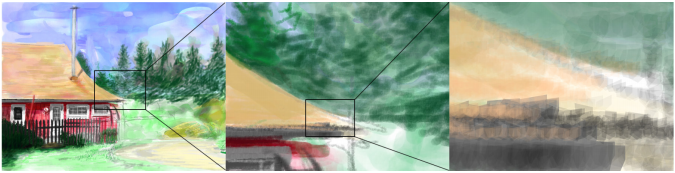
\includegraphics[width=0.8\paperwidth]{f1.png}
        \caption{\footnotesize{A vector watercolor painting made with the
        interactive iPad painting application, displaying complex texture and
        color blending.  Insets zoom in to show stroke detail and resolution
        independence.}}
    \end{figure}
\end{frame}

\begin{frame}
    \frametitle{Introduction}
    The problem:
    \begin{itemize}
        \item There have been great advances in digital painting;
        \item There remains a large contingent of traditional media artists;
        \item The wide range of complex textures and qualities that can be
        created using traditional media can be difficult to match digitally.
    \end{itemize}
    The goal:
    \begin{itemize}
        \item Not to exactly duplicate traditional watercolor painting;
        \item Create a range of dynamic behaviors which can achieve a similar
        style, process and result;
        \item Simultaneously maintain a unique character as well.
    \end{itemize}
\end{frame}

\begin{frame}
    \frametitle{Related Work}
    \begin{itemize}
        \item Most existing work is focused on the automatic conversion of
        photographs into watercolor paintings;
        \item Some existing commercial applications attempt to mimic a
        water-color style effect;
        \item Interactive digital oil painting has been attempted as well;
        \item Watercolor painting has been generally found to be very complex
        to model appropriately.
    \end{itemize}
\end{frame}

\begin{frame}
    \frametitle{Algorithm}
    \begin{itemize}
        \item The general intuition is that watercolor stroke effects are
        generally sparse;
        \item Each particle in a real watercolor paint can be thought of as
        taking a random walk;
        \item The aggregate behavior is that of watercolor paint.
    \end{itemize}
\end{frame}

\begin{frame}
    \frametitle{Algorithm}
    \begin{figure}
        \centering
        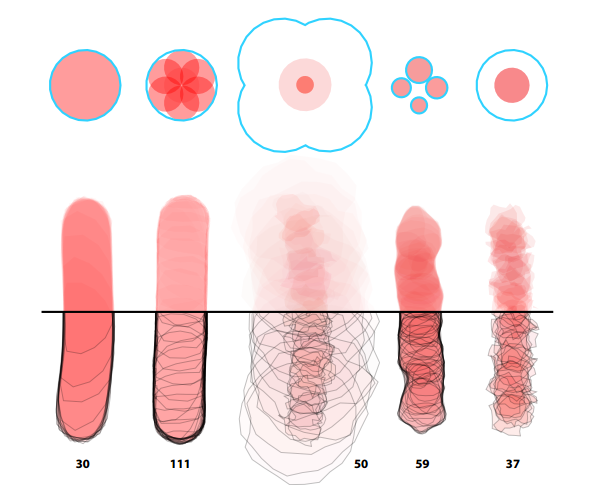
\includegraphics[width=0.6\paperwidth]{f2.png}
        \caption{\footnotesize{Initial splat configurations and resulting
        stroke for each brush type.}}
    \end{figure}
\end{frame}

\begin{frame}
    \frametitle{Algorithm - Paint Initialization}
    \begin{itemize}
        \item During stroke input, stamps are placed in uniform path length
        increments along the stroke path;
        \item Each stamp is a set of one or more spats arranged according to
        the current brush type;
        \item At each stamp, an amount of water is also added to the canvas;
        \item The result is a ``wet map'' consisting of a 2D grid of cells
        which are currently wet and will stay wet for a certain amount of time.
    \end{itemize}
\end{frame}

\begin{frame}
    \frametitle{Algorithm - Pigment Advection}
    \begin{itemize}
        \item Pigment advection refers to the random walk behavior of
        individual particles in real watercolor paint flow;
        \item Once a splat's vertices have all been updated, its opacity
        is recomputed by conserving the ``amount of pigment'';
        \item After all the splats have been updated, the wet map is updated
        as well by decrementing all the non-zero values stored in it.
    \end{itemize}
\end{frame}

\begin{frame}
    \frametitle{Algorithm - Pigment Advection}
    \begin{figure}
        \centering
        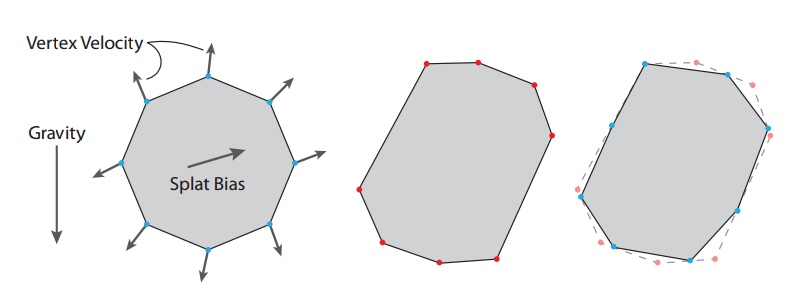
\includegraphics[width=0.8\paperwidth]{f3.png}
        \caption{\footnotesize{Each spat's motion is dictated by a per-vertex
        velocity, a splat bias, and a global gravity.}}
    \end{figure}
\end{frame}

\begin{frame}
    \frametitle{Algorithm - Sampling Management}
    \begin{itemize}
        \item Different advection directions of each vertex in a spat can
        result in unrealistically straight hard edges;
        \item Two strategies deal with this issue;
        \item First, the motion of vertices is constrained so that a spat
        is not too far from it's neighbors;
        \item Second, each splat's boundaries are periodically re-sampled;
        \item Both strategies smooth the splat boundary and limit polygonal
        artifacts;
    \end{itemize}
\end{frame}

\begin{frame}
    \frametitle{Algorithm - Lifetime Management}
    \begin{itemize}
        \item A splat has three stages of life: flowing, fixed, and dried;
        \item The addition of water can re-wet splats to achieve certain
        effects;
        \item The age of the splat also determines the impact of the
        granulation texture.
    \end{itemize}
\end{frame}

\begin{frame}
    \frametitle{Algorithm - Brush Types}
    \begin{itemize}
        \item The authors implemented five brush types that produce a variety
        of characteristic watercolor strokes;
        \item Many more variations are possible;
        \item The key differences are the splats per stamp and the orientation
        of the splats within the stamp.
    \end{itemize}
\end{frame}

\begin{frame}
    \frametitle{Algorithm - Brush Types}
    \begin{figure}
        \centering
        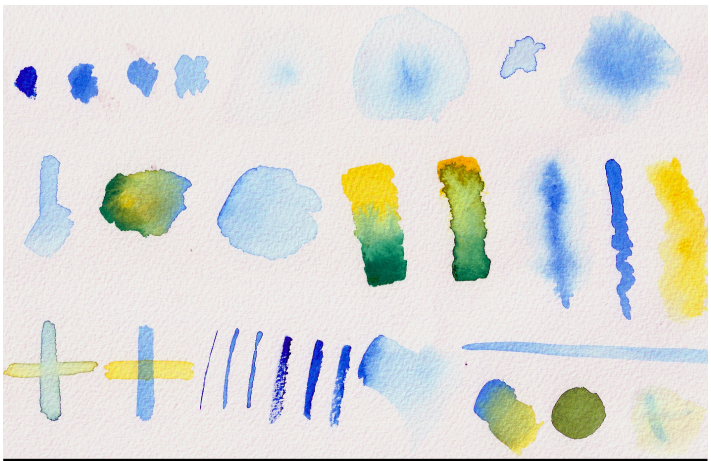
\includegraphics[width=0.8\paperwidth]{f4-1.png}
        \caption{\footnotesize{A comparison of similar strokes made with real
        watercolor paint.}}
    \end{figure}
\end{frame}

\begin{frame}
    \frametitle{Algorithm - Brush Types}
    \begin{figure}
        \centering
        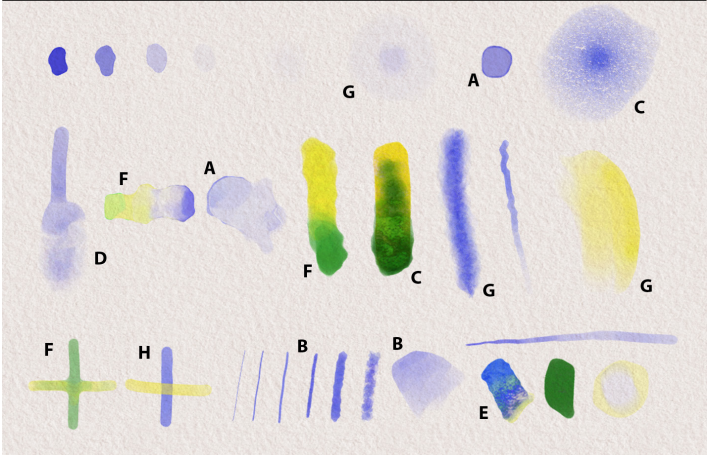
\includegraphics[width=0.8\paperwidth]{f4-2.png}
        \caption{\footnotesize{A comparison of similar strokes made with the
        algorithm.}}
    \end{figure}
\end{frame}

\begin{frame}
    \frametitle{Application}
    \begin{itemize}
        \item The authors have made a number of considerations to make the
        application usable;
        \item The authors have produced both desktop and iPad applications
        implementing the algorithm.
    \end{itemize}
\end{frame}

\begin{frame}
    \frametitle{Application - Interactive Rendering}
    \begin{itemize}
        \item The application uses OpenGL to render the splats and the dried 
        pigment buffer;
        \item The application uses a two-pass stencil buffer approach per splat
        \item This is due to the high overhead of the alternative -- repeated
        polygonal tessellation.
    \end{itemize}
\end{frame}

\begin{frame}
    \frametitle{Application - User Interface}
    \begin{itemize}
        \item The basic form of the desktop application presents the canvas
        alongside a GUI for controlling parameters;
        \item Users can paint with a mouse or Wacom tablet;
        \item In the iPad application, only finger-based input is available;
        \item No pressure or tilt sensitivity;
        \item Here, the canvas occupies the entire space.
    \end{itemize}
\end{frame}

\begin{frame}
    \frametitle{Application - Vector Output}
    \begin{itemize}
        \item When a canvas is saved, two output files are generated -- a
        bitmap of the rendered image as a PNG, and a vector representation of
        the splats;
        \item The SVG specification includes support for advanced features
        such as image filter effects and blend modes that could duplicate
        granulation texture shading math;
        \item Unfortunately no commonly available SVG viewers support these
        features.
    \end{itemize}
\end{frame}

\begin{frame}
    \frametitle{Algorithm - Vector Output}
    \begin{figure}
        \centering
        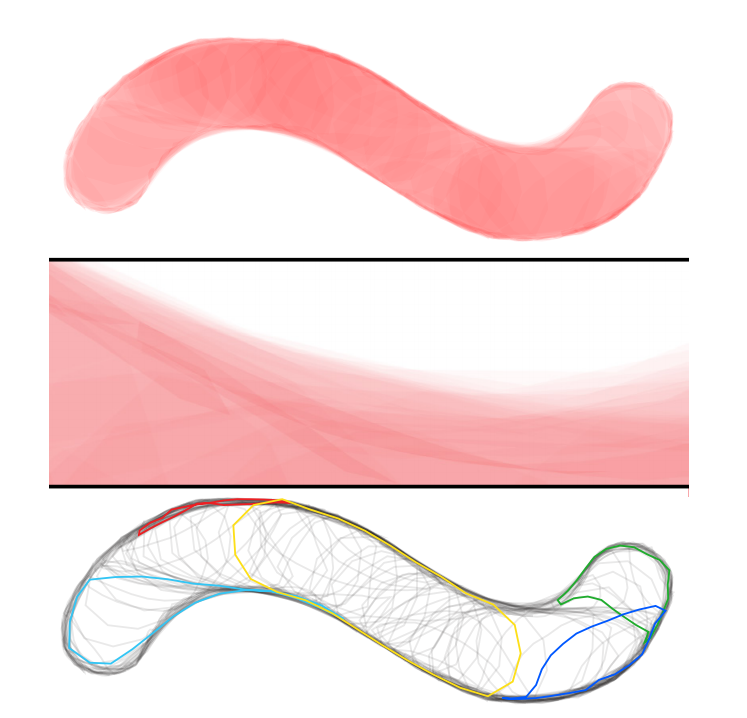
\includegraphics[width=0.5\paperwidth]{f5.png}
        \caption{\footnotesize{The vector output of a brush stroke made from
        left to right}}
    \end{figure}
\end{frame}

\begin{frame}
    \frametitle{Results}
    \begin{itemize}
        \item The authors have released the application as an iPad app;
        \item It interacts with the desktop version of Photoshop;
        \item The algorithm \& application has been used by many artists at
        different levels, with different styles, for different purposes.
    \end{itemize}
\end{frame}

\begin{frame}
    \frametitle{Results - Performance}
    \begin{itemize}
        \item Because the results are a vector file, the resolution of the
        image is not particularly important;
        \item The number of active splats dictates the performance of the
        application;
        \item Rendering can be improved by only drawing a subset of splats;
    \end{itemize}
\end{frame}

\begin{frame}
    \frametitle{Discussion - User Feedback}
    \begin{itemize}
        \item User reaction has been mixed;
        \item There seems to be a steep learning curve;
        \item Users have lamented the lack of typical features such as ``undo''
        and layers;
        \item This is similar to traditional watercolor paints.
    \end{itemize}
\end{frame}

\begin{frame}
    \frametitle{Algorithm - Vector Output}
    \begin{figure}
        \centering
        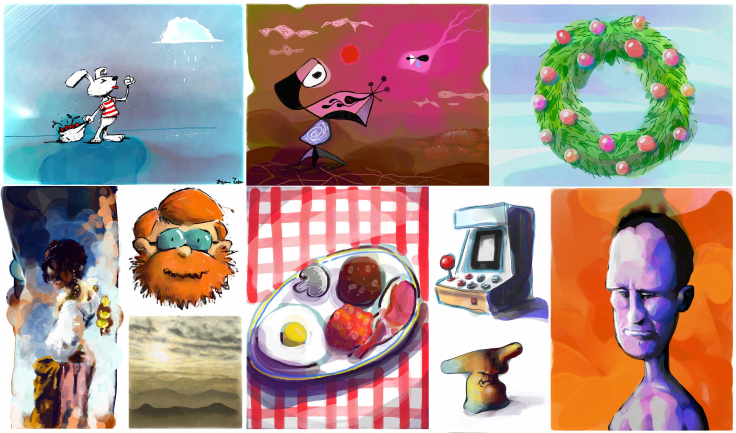
\includegraphics[width=0.8\paperwidth]{f6-1.png}
        \caption{\footnotesize{Examples of paintings by professional artists
        exhibiting different styles characteristic of watercolor painting.}}
    \end{figure}
\end{frame}

\begin{frame}
    \frametitle{Algorithm - Vector Output}
    \begin{figure}
        \centering
        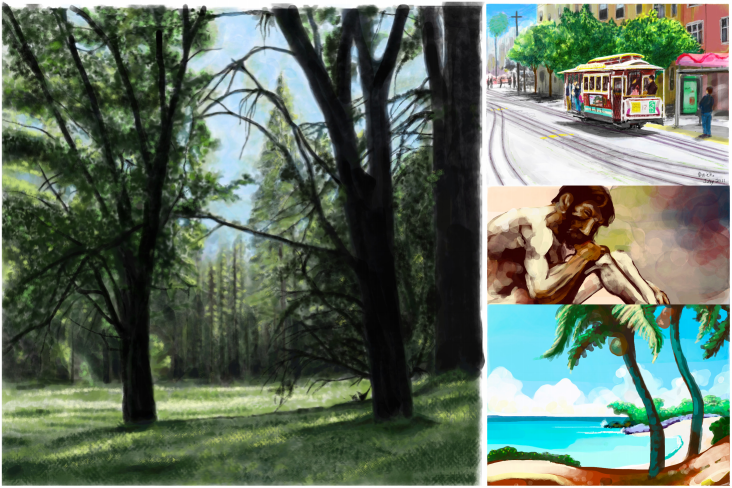
\includegraphics[width=0.8\paperwidth]{f6-2.png}
        \caption{\footnotesize{Examples of paintings by professional artists
        exhibiting different styles characteristic of watercolor painting.}}
    \end{figure}
\end{frame}

\begin{frame}
    \frametitle{Discussion - Limitations}
    \begin{itemize}
        \item The vector-based format reduces the overall complexity of the
        resulting image;
        \item The procedural approach to the pigment evolution makes it
        increasingly difficult to simulate the full range of paint behaviors,
        and the algorithmic complexity does not scale well;
        \item Obviously, the fidelity with which real paint can be faithfully
        reproduced with physical simulation is higher than with the simulated
        approach.
    \end{itemize}
\end{frame}

\begin{frame}
    \frametitle{Conclusion}
    \begin{itemize}
        \item The authors proposed a novel formulation of a dynamic and
        interactive paint engine that reproduces many of the important
        behaviors of watercolor paint;
        \item The authors implemented their algorithm as an application
        and publicly released it;
        \item Future work will continue to explore the range of effects
        that are possible with this type of algorithm.
    \end{itemize}
\end{frame}

\end{document}
